%%%%%%%%%%%%%%%%%%%%%
%   AMS packages    %
%%%%%%%%%%%%%%%%%%%%%
\documentclass{amsart}

\usepackage{amsmath}
\usepackage{amsxtra}
\usepackage{amscd}
\usepackage{amsthm}
\usepackage{amsfonts}
\usepackage{amssymb}
\usepackage{eucal}
\usepackage[all]{xy}
\usepackage{graphicx}
\usepackage{tikz-cd}
\usepackage{mathrsfs}
\usepackage{subfiles}
%\usepackage{mathpazo} not a huge fan
\usepackage{euler}
\usepackage{hyperref}
\usepackage{color}
\usepackage{longtable}
\usepackage{float}
\usepackage{caption}

\usepackage[colorinlistoftodos, textsize=tiny]{todonotes}
\def\listtodoname{List of Todos}
\def\listoftodos{\@starttoc{tdo}\listtodoname}

%\addtolength{\oddsidemargin}{-.5 in}
	%\addtolength{\evensidemargin}{-.4 in}
	%\addtolength{\textwidth}{1 in}
%
	%\addtolength{\topmargin}{0 in}
	%\addtolength{\textheight}{0 in}

\RequirePackage{color}
\definecolor{myred}{rgb}{0.75,0,0}
\definecolor{mygreen}{rgb}{0,0.5,0}
\definecolor{myblue}{rgb}{0,0,0.65}

%\usepackage{hyperref}
  %\hypersetup{colorlinks=true,citecolor=blue}

\usepackage{tikz}
\usepackage{tikz-cd}
\usetikzlibrary{matrix,arrows,decorations.pathmorphing}

%%%%%%%%%%%%%%%%%%%%%%% amsthm theorem styles %%%%%%%%
%%%%%%%%%%%%%%%

\theoremstyle{plain}
  \newtheorem{thm}{Theorem}[section]
  \newtheorem{prop}[thm]{Proposition}
  \newtheorem{lem}[thm]{Lemma}
  \newtheorem{cor}[thm]{Corollary}
	\newtheorem{claim}[thm]{Claim}
	\newtheorem{question}[thm]{Question}
	
\theoremstyle{definition}
  \newtheorem{defn}[thm]{Definition}
  \newtheorem{example}[thm]{Example}
  \newtheorem{exer}[thm]{Exercise}
  \newtheorem{ctexample}[thm]{Counterexample}
  \newtheorem{convention}[thm]{Convention}
	\newtheorem{conjecture}[thm]{Conjecture}
	
\theoremstyle{remark}
	\newtheorem{rem}[thm]{Remark}
  \newtheorem{note}[thm]{Notation}
  \newtheorem*{note*}{Notation}
  \newtheorem{case}{Case}
	
\numberwithin{equation}{section}

%%%%%%%%%%%%%%%%%%%%%%%%% custom commands %%%%%%%%%%%%%%%%%%%%%%%%%%%

\newcommand\nc{\newcommand}
\nc\on{\operatorname}
\nc\renc{\renewcommand}
\newcommand\ssec{\subsection}
\newcommand\sssec{\subsubsection}
\newcommand\bh{{\mathbb H}}
\newcommand\bn{{\mathbb N}}
\newcommand\bc{{\mathbb C}}
\newcommand\bbf{{\mathbb F}}
\newcommand\br{{\mathbb R}}
\newcommand\bq{{\mathbb Q}}
\newcommand\bp{{\mathbb P}}
\newcommand\bz{{\mathbb Z}}
\newcommand\ba{{\mathbb A}}
\newcommand\bk{{\Bbbk}}

\newcommand\sco{{\mathscr O}}

\newcommand{\id}{\mathrm{id}}
\newcommand\im{\text{im }}
\newcommand\coker{\text{coker}}
\newcommand\gal{\mathrm{Gal}}

\DeclareMathOperator{\ord}{ord}
\DeclareMathOperator{\sym}{Sym}

%%%%%%%%%%%%%%%%%%%%% csurfaces custom commands %%%%%%%%%%%%%%%%%%%%%%%%%

\DeclareMathOperator\di{Div}
\newcommand\bida{a}
\newcommand\bidb{b}
\newcommand\pdeg{\delta}
\newcommand\hirz{\mathbb{F}}
\newcommand\mss{\mathscr{S}}

\DeclareMathOperator{\supp}{Supp}
\DeclareMathOperator{\initial}{in_\prec}
\DeclareMathOperator{\gin}{gin}
\DeclareMathOperator{\Eff}{Eff}
\DeclareMathOperator{\sat}{sat}
\DeclareMathOperator{\newspan}{span}
\DeclareMathOperator{\proj}{Proj}
\DeclareMathOperator{\spec}{Spec}
\DeclareMathOperator{\Te}{T_=}
\DeclareMathOperator{\Tp}{T_+}
\DeclareMathOperator{\Tm}{T_-}
\DeclareMathOperator{\num}{p}
\DeclareMathOperator{\den}{q}
\DeclareMathOperator{\lcm}{lcm}
\DeclareMathOperator{\Pic}{Pic}
%\captionsetup[table]{belowskip = 4pt}

\makeatletter
\newcommand{\customlabel}[2]{%
   \protected@write \@auxout {}{\string \newlabel {#1}{{#2}{\thepage}{#2}{#1}{}} }%
   \hypertarget{#1}{#2}
}
\makeatother

%%%%%%%%%%%%%%%%%%%%%%%%%%%%%% title %%%%%%%%%%%%%%%%%%%%%%%%%%%%%%%%

\title{Canonical rings of rational divisors on projective space and Hirzebruch surfaces}

\author{Aaron Landesman}
\address[Aaron Landesman]{Department of Mathematics, Harvard University}
\email{aaronlandesman@college.harvard.edu}

\author{Peter Ruhm}
\address[Peter Ruhm]{Department of Mathematics, Stanford University}
\email{pruhm@stanford.edu}

\author{Robin Zhang}
\address[Robin Zhang]{Department of Mathematics, Stanford University}
\email{robinz16@stanford.edu}

\date{\today}

%%%%%%%%%%%%%%%%%%%%%%%%%%%%% document %%%%%%%%%%%%%%%%%%%%%%%%%%%%%%

\begin{document}

\begin{abstract}
 	Bounding generator and relation degrees of general $\bq$-divisors
	on projective spaces $\bp^n$ and Hirzebruch surfaces.
\end{abstract}

\maketitle

%%%%%%%%%%%%%%%%%%%%%%%%%%%% Introduction %%%%%%%%%%%%%%%%%%%%%%%%%%%%%%%

\section{Introduction}
\todo{Clean up this stuff on siegel modular forms, hilbert modular forms, say something about hasse keel program, canoncical rings studied before}

\todo{Might be reasonable to think about higher dimensional rational varieties that are similar to these hirzebruch surfaces.}

\todo{The following stuff is almost nonsensical now, will be edited much more soon}

Hasse keel program, birational map from $proj R(K + \Delta)$ to $M_2$, they showed finite generation, we're giving explicit generators and bounds.

The work in this paper also yields bounds for certain rings of Hilbert modular forms. Recall that a Hilbert modular form is a generalization of modular forms to multiple variables.

Siegel modular forms are a generalization of modular forms on the Siegel upper half plane to automorphic forms on the Siegel upper half space. Explicitly, the Siegel uper half space is $\mathscr H \cong \bc^n/\Lambda$ and siegel modular forms are functions on $Sp_{2g} \backslash \mathscr H.$ Then, modular functions are differentials invariant under the action of $Sp_{2g}$. In the case that $\Gamma \backslash \mathscr H$.

Example: the Siegel 2-upper half plane $\bc^2/\Lambda$ Note that $\bc^2/\Lambda$ is algebraic if and only if there exists a hermitial form on $\Lambda$. Then, $Sp_{2g}$ acts on algebraic lattices. The quotient by this gives you the space of abelian varieties. This might be an open subset of projective space, according to David, 65$\%$.

\section{Background}

\begin{defn}
\label{defn:lower-approximation}
If $\alpha \in \br$, then a rational number $\frac{c}{k} \leq \alpha
$ (written in reduced form with $c \in \bz, k \in \bn$) is a
\textbf{best lower approximation} to $\alpha$ if there does not
exist $\frac{c'}{k'}\in \mathbf{Q}$ such that $0 < k'< k$ and
$\frac{c}{k} \le \frac{c'}{k'} \le \alpha$. 
\end{defn}

\begin{rem}
\label{rem:lower-approximation}
Note that all integers less than or equal to $\lfloor \alpha \rfloor$
are best lower approximations to $\alpha$. Also, if $\alpha \ge 0$,
then the non-negative best lower approximations of
$\alpha$ form a finite sequence
\[
	0 = \frac{c_0}{k_0} < \frac{c_1}{k_1} < \ldots < \frac{c_r}{k_r} = \alpha.
\]

\noindent
Figure \ref{fig:s14/5-lattice} gives a pictorial representation of the positive best lower approximations of $\alpha = \frac{14}{5}$.
\end{rem}

\begin{figure}
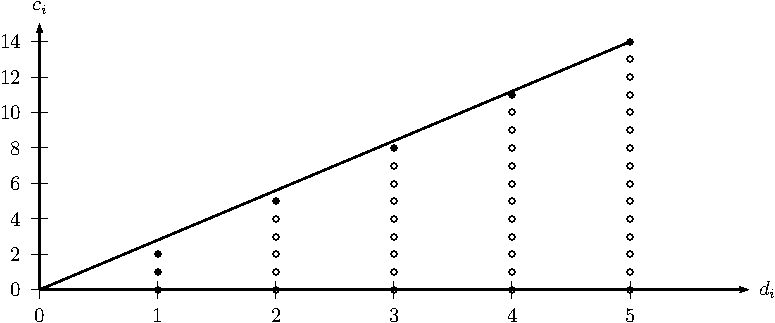
\includegraphics{pics/spin-lower-approximations-pic-pics.pdf}
\caption{This figure shows each non-negative best lower
approximation of $\frac{14}{5}.$ Each ``$\bullet$'' denotes a best
lower approximation and each ``$\circ$'' denotes a lattice point
below $5y=14x$ which is not a best lower approximation.  Note that
the non-negative best lower approximations generate the monoid of
lattice points in the first quadrant satisfying  $5y \le 14x$, with
the operation $(a_1, b_1)(a_2, b_2)\mapsto (a_1 + a_2, b_1 + b_2)$.}
\label{fig:s14/5-lattice}
\end{figure}

\ssec{Notation}
\begin{convention}
Write
\begin{align*}
	D = \sum_{i=1}^{n}\alpha_i D_i.
\end{align*}
where $\alpha_i \in \bq$. \todo{Peter: What are the $D_i$'s.}
\end{convention}

\begin{convention}
Let $\{x_0, \ldots, x_m\}$ be coordinates for $\bp^m$. Let
$\vec{v} = (v_0, \ldots, v_m) \in \br^{m + 1}$. Then write
\[
	x_{\vec{v}} := \prod_{i = 0}^{m} x_i^{v_i}
\]
\end{convention}

\section{Lemmas for Generation and Relations}

\begin{prop}
\label{prop:cone-generation}
Let $n,t \in \bz,$ let $\alpha_1, \ldots, \alpha_n \in \bq$ and let $k_i^j \in \bz$ with $1 \leq i \leq n, 1 \leq j \leq t.$ Define
\begin{align*}
	\Sigma = \{(d, c_1, \ldots, c_n) \in \bz^{n+1} : c_i \geq - d \alpha_i,1 \leq i \leq n \text{ and } \sum_{i=1}^{n}k_i^j = 0, 1 \leq j \leq t\}
\end{align*}

\noindent
Suppose $e_1, \ldots, e_t \in \Sigma$ with $e_i = (\pdeg_i, c_1^i,
\ldots, c_n^i)$ are a set of {\bf extremal rays} of $\Sigma$,
meaning that the $\Sigma$ is contained in the $R_{\geq 0}$ span of
$e_1, \ldots, e_t$.  Then, as a semigroup, $\Sigma$ is generated by
elements whose first coordinate is less than $\sum_{i = 1}^{n} \pdeg_i$
. Furthermore, every element $\sigma \in \Sigma$ can be written in
a canonical form $\lambda + \sum_{i=1}^{t} w_i e_i,$ with the first
coordinate of $\lambda$ less than $\sum_{i=1}^{t}\pdeg_i$ and $w_1,
\ldots, w_t \in \bz$.
\end{prop}

\begin{proof}
By assumption, $\sigma \in \Sigma$ as $\sigma = \sum_{i=1}^{t} r_i e_i$ with $r_i \in \br$. Let $\{r\} := r - \lfloor r \rfloor$ denote the fractional part of $r$. Let $\lambda = \sum_{i=1}^{t}\{r_i\}$. Hence, we can write $\sigma = \lambda + \sum_{i=1}^{t}\lfloor r_i \rfloor e_i.$ Hence, $\sigma$ lies in the $\bz_{\geq 0}$ span of $\lambda, e_1,\ldots, e_t$, which all have first coordinate less than $\sum_{i=1}^{t}r_i$. Therefore, $\Sigma$ is generated by elements whose first coordinate is less than $\sum_{i=1}^{t}r_i$.
\end{proof}

\begin{lem}
\label{lem:composite-map}
Let $D = \sum_{i=1}^{n}\alpha_i D_i$ where $D_i = V(f_i)$. Suppose we have a surjection $\phi: \bk[x_1,x_2,\ldots, x_r] \rightarrow R_D$ given by $x_i \mapsto p_i(f_1, \ldots, f_n),$ where $p_i$ is a monomial in $f_1,\ldots, f_n$. Let $\bida_1, \ldots, \bida_n, \bidb_1, \ldots, \bidb_n \in \bz_{\geq 0}.$ Then, define
\begin{align*}
	\Sigma = \langle u^d z_1^{c_1} \cdots z_n^{c_n} : c_i \geq -d \alpha_i, \sum_{i=1}^{n} \bida_i c_i = \sum_{i=1}^{n} \bidb_i c_i. \rangle 
\end{align*}
In this case, we can factor $\phi$ through maps $\chi, \psi$ defined by
\todo{Make this have mapsto on bottom}
\[
\begin{tikzcd}
\bk[x_1,\ldots, x_r] \ar {r}{\chi} & \bk[\Sigma] \ar {r}{\psi} & R_D \\
x_i \ar r & u^{d_i}z_1^{c_{i1}} \cdots z_n^{c_{in}} \ar r & u^{d_i}f_1^{c_{i1}} \cdots f_n^{c_{in}}
\end{tikzcd}
\]
Assuming $\chi$ is surjective, the minimal degree of generation of $\ker \phi$ is at most the maximum of the minimal degree of generation of $\ker \chi$ and the minimal degree of generation of $\ker \psi$.
\end{lem}
\begin{proof}
Note that we have an exact sequence
\[
\begin{tikzcd}
0 \ar r & \ker \chi \ar r & \ker \phi \ar r & \ker \psi \ar r & 0.
\end{tikzcd}
\]
To see this, note that the left map is an inclusion because $\phi = \chi \circ \psi$. Next, the right map, given by $\chi|_{\ker \phi}:\ker \phi \rightarrow \ker \psi$ is a surjection, again because $\phi = \chi \circ \psi$. The composition of the two maps is $0$ by definition of the kernel of $\chi$. Finally, if $a \in \ker \phi$ and $a$ lies in the kernel of the right map, then by definition $\chi(a) = 0$.
\end{proof}

\begin{lem}
\label{lem:bound-ker-chi}
Retaining the notation of Lemma ~\ref{lem:composite-map}, if $\Sigma$ has extremal rays $e_1,\ldots, e_r$ in degrees $d_1, \ldots, d_r$ then $\ker \chi$ has a system of generators in degrees at most $2(\sum_{i=1}^{r}d_r-1)$.
\end{lem}
\begin{proof}
Since $e_1, \ldots, e_r$ are extremal rays, by Proposition ~\ref{prop:cone-generation}, every element $\sigma \in \Sigma$ can be written in a canonical form $\lambda + \sum_{i=1}^{r}e_i$. Now, letting $\lambda_0 := 0,\lambda_1, \ldots, \lambda_m$ be all elements of $\Sigma$ so that we can write $\lambda_i = \sum_{i=1}^{r}\bida_i e_i$ with $0 \leq \bida_i < 1$ for all $i$. Then, for any $1 \leq i \leq j \leq m,$ we can write $\lambda_i + \lambda_j$ in the above canonical form, yielding a relation in degree at most $\deg \lambda_i + \deg \lambda_j \leq 2 \cdot \left( \sum_{i=1}^{r}d_r -1 \right).$ Furthermore, these relations generate all relations, as one can apply a sequence of these relations to put any $\sigma \in \Sigma$ into canonical form.
\end{proof}


\section{Canonical Rings on Projective Space}
In this section, we bound the degrees of generators and relations for divisors on $\bp^m$, for all $m \geq 1$. The $\bp^1$ case was covered in \cite{dorney:canonical}.

\ssec{Preliminaries on Projective Space}

For the remainder of this section, we shall fix $m \geq 1$ and choose an isomorphism $\bp^m \cong \proj V$ so that $x_0,\ldots, x_m$ form a basis for $V$.  We will think of $x_i$ as a rational section of $H^0(\bp^m, \sco_{\bp^m})$ of degree 1.


Write
\begin{align*}
	D = \sum_{i=0}^{n}\alpha_i D_i.
\end{align*}
where $\alpha_i \in \bq$ and $\deg D_i = \bida_i$. Let $f_i$ be Cartier divisors such that $D_i = V(f_i)$. \todo{Should this say $D_i$ is a Cartier divisor.  Also should we say $\deg(f_i)= \bida_i$ rather than $\deg(D_i)$.}
We shall further assume that (after reordering) $f_0,\ldots, f_{m}$ form a basis for degree one rational functions on $\bp^m$. \todo{Peter: Make reference to ghost points here?}

\begin{prop}
\label{prop:pm-span-and-basis}
The functions $u^d \cdot \prod_{i=1}^n f_i^{c_i}$ satisfying
\begin{align}
\label{align:pm-span}
\sum_{i=1}^{n} c_i \cdot \bida_i \cdot f_i = 0 && \text{ and } &&c_i \geq \lfloor \alpha_i d\rfloor	
\end{align}

\noindent
form a spanning set for $H^0(\bp^m, dD)$ over $k$. Furthermore, functions 
of the form $u^d \cdot \prod_{i=1}^n f_i^{c_i}$ satisfying
\begin{align}
\label{align:pm-basis}
c_i = -\lfloor d\alpha_i \rfloor && \text{ for } && i > m
\end{align}

\noindent
form a basis for $H^0(\bp^m, dD)$ over $k$.
\end{prop}

\begin{proof}
By definition of $H^0(\bp^m,dD)$, functions satisfying conditions 
~\eqref{align:pm-span} lie in $H^0(\bp^m,dD)$. To complete the proof, it suffices to check functions satisfying conditions ~\eqref{align:pm-basis} form a basis of $H^0(\bp^m,dD)$. Note that there $\binom{m+ \lfloor dD \rfloor }{m}$ functions satisfying condition ~\eqref{align:pm-basis}. However we know $h^0(\bp^m,dD) = \binom{m+ \lfloor dD \rfloor }{m},$ so it suffices to show that those functions satisfying condition ~\eqref{align:pm-basis} are independent. This follows from the assumption that $f_0,\ldots, f_n$ form a basis of degree 1 rational functions, and so degree $\lfloor d \deg D \rfloor $ monomials in $f_0,\ldots, f_n$ form a basis of degree $\lfloor d \deg D \rfloor $ rational functions.
\end{proof}

We first restrict attention to the case $n=1$, so $D = \alpha D_i$.

\ssec{One point on Projective Space}
\label{ssec:proj-one-point}

\begin{rem}
Remark about how we can assume divisor only consists of hyperplanes
by taking the Veronese embedding.
\todo{write}
\end{rem}

\begin{defn}
\label{defn:vec-sum}
For $\vec{v} \in \br^n$, denote $\deg \vec{v} := \sum_{i = 0}
^n v_i$ (i.e. the taxicab metric).
Let $\mss_i := \{\vec{v} \in \bz_{\geq 0}^{m + 1} \; : \;
\sum_{i = 0} ^{m + 1} v_i = c_i\}$ be the set of $\bz_{\geq 0}
^{m + 1}$-vectors with sum of components equal to $c_i$.
\end{defn}

\begin{defn}
\label{defn:vec-order}
Let $\vec{v}, \vec{w} \in \br^n$ be two vectors. Let $i$
be the right-most coordinate such that $v_i$ is nonzero
and $j$ be the left-most coordinate such that $w_j$ is
nonzero. Define $\vec{v} \prec \vec{w}$ if $i \leq j$.
\end{defn}


\begin{thm}
\label{thm:proj-one-point}
Let $X = \bp^m$ with $\{x_0, \ldots, x_m\}$ a coordinate system for
$\bp^m$. Let $D = \alpha H$, with $\alpha = \frac{p}{q} \in \bq$
and $H = V(x_k)$ a hyperplane of $\bp^m$, be a divisor on $\bp^m$.
Let
\[
	0 = \frac{c_0}{d_0} <
	\frac{c_1}{d_1} < \ldots < \frac{c_r}{d_r} = \frac{p}{q}
\]

\noindent
be the best lower approximations of $\alpha$. Then the
canonical ring
\[
	R_D := \bigoplus_{d \geq 0} H^0(\bp^m, \lfloor dD \rfloor)
\]

\noindent
has a minimal presentation consisting of the $\sum_{i = 0}^{r}
{{m + i} \choose {i}}$ generators $F_i^{\vec{v}} := \frac{u^{d_i}
x^{\vec{v}}}{x_k^{c_i}}$ where $\vec{v} \in \bz_{\geq 0}^{m + 1}$
such that $\sum_{j = 0}^{m} v_j = c_i$. Furthermore, it has $z$
many \todo{how many?} relations of the following two types.

For each $(i, j)$ with $j \geq i + 2$ and each $\vec{v} \in \mss_i,
\vec{w} \in \mss_j$, there is a relation of the form either
\begin{flalign*}
	&G_{i, j}^{\vec{v}, \vec{w}} = F_i^{\vec{v}} F_j^{\vec{w}}
	- \prod_{\vec{y} \in \mss_{h_{i, j}}} (F_{h_{i, j}}^{\vec{y}})
	^{g_{\vec{y}}} &(i < h_{i, j} < j) \\
	\text{or} \\
	&G_{i, j}^{\vec{v}, \vec{w}} = F_i^{\vec{v}} F_j^{\vec{w}}
	- \prod_{\substack{\vec{y} \in \mss_{h_{i, j}} \\ \vec{z} \in
	\mss_{h_{i, j} + 1}}} (F_{h_{i, j}}^{\vec{y}})^{g_{\vec{y}}} \;
	(F_{k_{i, j} + 1}^{\vec{z}})^{g'_{\vec{z}}}
	&(i < h_{i, j} < h_{i, j} + 1 < j).
\end{flalign*}

Furthermore, there are the relations for each $(i, j)$ with
$j = i$ or $j = i + 1$ and each $\vec{v} \in \mss_i, \vec{z} \in
\mss_j$ with $\vec{v} \not\prec \vec{z}$ (see Definition
~\ref{defn:vec-order}) of the form 
\begin{align*}
	&L_{i, j}^{\vec{v}, \vec{z}} = F_i^{\vec{v}} F_j^{\vec{z}}
	- F_i^{\vec{y}} F_j^{\vec{z}} \\
\end{align*}

\noindent
where $\vec{y}$ and $\vec{z}$ are the unique
vectors in $\mss_i$ and $\mss_j$, respectively, such that $\vec{y}
\prec \vec{z}$.
\end{thm}

\begin{proof}
We know $\left\{F_{0}^{\vec{v}} : \deg \vec{v} = \left\lfloor
\frac{p}{q} \right\rfloor \right\}$ are minimal generators in
degree $1$. Now let $i > 0$. Suppose $F_i^{\vec{v}}$ were not
minimal for some $\vec{v} \in \mss_i$. Then $F_i^{\vec{v}} =
F_{s}^{\vec{y}} F_{t}^{\vec{z}}$ for some $s, t \in \bn$ and
$\vec{y}, \vec{z} \in \bz_{ \geq 0}^{m + 1}$. In particular, we see
that 
\begin{align*}
	&d_i = s + t \\
	&c_i = \deg \vec{v} = \deg \vec{y} + \deg \vec{z}
\end{align*}

\noindent
so $\frac{c_i}{d_i}$ is the mediant of the rational numbers
$\frac{\deg \vec{y}}{s}, \frac{\deg \vec{z}}{t}$ which both
do not exceed $\alpha$. One of $\frac{\deg \vec{y}}{s},
\frac{\deg \vec{z}}{t}$ must be at least $\frac{c_i}{d_i}$
and $s$ and $t$ are both less than $d_i$, so we have a contradiction 
of $\frac{c_i}{d_i}$ being a best lower approximation of $\alpha$
(see Definition ~\ref{defn:lower-approximation}).

Now we show that no further generators are necessary. As done in
the proof of the $\bp^1$ case by O'Dorney \cite[Theorem 6]
{dorney:canonical}, each lattice point $(\beta, \gamma) \in
\bz_{\geq 0}^2$ such that $\gamma \leq \beta \alpha$ is a non-negative
linear combination of $(d_h, c_h)$ and $(d_{h + 1}, c_{h + 1})$ for
some $h \in \{0, \ldots, r\}$. Let $(\beta, \gamma) = \ell_1
(d_h, c_h) + \ell_2 (d_{h + 1}, c_{h + 1})$ for $\ell_1, \ell_2 \in
\bz_{\geq 0}$. Consequently, any element $\frac{u^{\beta}
x^{\vec{v}}} {x_k^{ \gamma}} \in R_D$ is expressible as
\begin{align*}
	\frac{u^{\beta} x^{\vec{v}}} {x_k^{\gamma}} = \left(\frac{u^{d_h}}
	{x_k^{c_h}}\right)^{\ell_1} \left(\frac{u^{d_{h + 1}}}
	{x_k^{c_{h + 1}}}\right)^{\ell_2} x^{\vec{v}}.
\end{align*}

\noindent
We can break $\vec{v}$ into a sum of $\ell_1$ many vectors
$\vec{w}_{(j)}$ in $\mss_2$ and $\ell_2$ many vectors $\vec{z}_{(k)}$
in $\mss_2$ to give a decomposition
\begin{align*}
	\frac{u^{\beta} x^{\vec{v}}} {x_k^{\gamma}}	= \prod_{\lambda = 1}
	^{\ell_1} \frac{u^{d_h} x^{\vec{w}_{(\lambda)}}} {x_k^{c_h}}
	\prod_{\lambda = 1}^{\ell_2} \frac{u^{d_{h + 1}} x^{\vec{z}_{(\lambda)}}}
	{x_k^{c_{h + 1}}}
\end{align*}

\noindent
consisting of products of generators $F_h^{\vec{y}_{(\lambda)}}$
and $F_{h + 1}^{\vec{z}_{(\lambda)}}$ which are in the form
prescribed in the theorem statement.

In particular, if $j \geq i + 2$ then $F_i^{\vec{v}} F_j^{\vec{w}}$
has a decomposition of this form for some $h_{i, j}$. We also have
that $i \leq h_{i, j} < j$ since $(d_i + d_j, c_i + c_j)$ is in the
$\bz_{\geq 0}$-span of $(d_{h_{i, j}}, c_{h_{i, j}})$ and
$(d_{h_{i, j} + 1}, c_{h_{i, j} + 1})$. Furthermore, we have that
$h_{i, j} \neq i$ is equivalent to the proof given by O'Dorney
\cite[Theorem 6]{dorney:canonical}. This gives the relations
$G_{i, j}^{\vec{v}, \vec{w}}$.

The application of $G_{i, j}^{\vec{v}, \vec{w}}$ can be used
to transform any monomial in the $F_i^{\vec{v}}$'s involving
indices that differ by more than $1$ to a monomial in the $F_i
^{\vec{v}}$'s involving indices that differ by at most $1$.

Furthermore, we have relations

\todo{relations}
Canonical form of 
\[
	\prod_{\substack{0 \leq i \leq m + 1 \\ \vec{y}
	\in \mss_i}} (F_i^{\vec{y}})^{g_{\vec{y}}}
\]

\noindent
where the indices with
some nonzero $g_{\vec{y}}$ are consecutive.
\end{proof}


\todo{change thm to be inductive for adding pts, giving result on
effective divisors}
\todo{remark on not doing two points}

\ssec{Bounds for Arbitrary Divisors on Projective Space}

\begin{rem}
When $\langle f_1, \ldots, f_r \rangle = \langle x_0, \ldots, x_n \rangle$ (the irrelevant ideal), we may directly use the hypersurface method by considering $x_0, \ldots, x_n$ instead of the $f_i$'s. However, when $\sqrt{\langle f_1, \ldots, f_r \rangle} = \langle x_0, \ldots, x_n \rangle$ (or the saturation), we cannot obtain the same result from our modification of O'Dorney's method as seen in Example ~\ref{eg:radical}. Instead we must use ghost points and hypersurfaces.
\end{rem} \todo{Peter: What is the purpose of this remark?  The only method we have extends to ghost points so that this is satisfied.}

\begin{example}
\label{eg:hyperplane}
Suppose $D = \frac{1}{2}H_0 - \frac{1}{3}H_1$ where $H_0 = V(x_0), H_1 = V(x_1)$ are two coordinate hyperplanes in $\bp^2$. Then, $R_D$ has generators in degree $2$ and $3$ which can be written as $u^2 \frac{x_1}{x_0}, u^3 \frac{x_1}{x_0}.$ In fact, for all degrees less than $5$ the elements of $R_D$ can all be expressed as rational functions in $x_0, x_1$. However, in degree $6$, there is the rational function $\frac{x_1^2 x_2}{x_0^3}.$ Since this involves $x_2$, it must be a generator.

This example generalizes slightly to any divisor of the form $D = \frac{1}{k}H_0 - \frac{1}{k+1}H_1 \in \di \bp^2 \otimes \bq,$ with $k \in \bn$, showing that there will always exist a generator in degree $a(a+1).$

This example further generalizes to the following situation: Suppose $D = \sum_{i=1}^{n} \frac{\num_i}{\den_i}D_i \in \di \bp^m \otimes \bq,$ where $\deg D_i = \bida_i$ and \todo{Peter: We need some condition that $D_i$'s be irreducible divisors or something.} $\deg D = \frac{1}{\lcm_{1 \leq i \leq n}(\den_i \cdot \bida_i)}$. Then, if $D_i = V(f_i)$ where all $f_i$ can be written as a polynomial function in $x_0, \ldots, x_{m-1},$ we have $R_D$ always has a generator in degree $\lcm(\den_i \cdot \bida_i)$.
\end{example}

\begin{rem}
\label{rem:ghost-motivation}
Example ~\ref{eg:hyperplane} shows that the naive generalization of ~\cite[Theorem 8]{dorney:canonical} of generation in degree at most $\sum_{i=1}^{n}\ell_i$ cannot possibly hold. The reason for this is that the divisors may ``be contained in a hyperplane,'' i.e., be expressable as functions in $m$ of the $m+1$ variables on $\bp^m$. This problem can easily be circumvented by adding in ``ghost points.'' That is, we may add divisors of the form $0 \cdot H_i$ to $D$, and reorder so that if $D = \sum_{i=1}^{n}\alpha_i V(f_i)$, then $f_0, \ldots, f_n$
\end{rem}

\begin{example}
\label{eg:radical}
In this example, we show that it is still, in general, necessary to add ghost points, even when the irreducible components of a divisor are not all contained in a hyperplane.

Consider $\frac{-1}{5}V(x_0^2 + x_1^2 + x_2^2) + \frac{1}{7}V(x_0^2 + x_1^2 + x_3^2) + \frac{1}{17}V(x_0^2 + x_2^2 + x_3^2) + \frac{1}{596}V(x_1^2 + x_2^2 + x_3^2)$. In degree $355216 = 5* 7 * 17 * 596$, this has dimension $10$. 
\todo{Clarify what this example means by the lattice approach}
However, we possibly use the lattice approach, as all lower degrees only have dimension 1. In fact, we may construct similar examples using any set of degree $n$ divisor with very small degree.
\end{example}
\todo{construct class of additional examples}
\todo{The example above needs to be changed because $x_0^2$ can be replaced by $2x_0$}

We now move on offer bounds on generators and relations of $R_D$ for a general divisor $D$ on $\bp^m$.

Let $D = \sum_{i=1}^n \alpha_i C_i$ for curves $C_i$ on $\mathbb{P}^m$ and let $f_i$ be homogeneous polynomials in $x_0, \ldots, x_m$ such that $C_i = v(f_i)$ for all $i$; suppose $\deg(f_i) = a_i$. 
\begin{lem} \label{P-m-generators}
$R_D$ is generated in degree at most $\sum_{i=1}^n \ell_i a_i$.
% and relations in degree at most  .\todo{insert numbers}
\end{lem}
\begin{proof}
Let 
\begin{align}\label{eqn:Sigma-def}
	\Sigma = \{(d, c_1, \ldots, c_n) \in \bz^{n+1} : c_i \geq - d \alpha_i, \; 1 \leq i \leq n, \text{ and } \sum_{i=1}^{n}k_i^j = 0, 1 \leq j \leq t\}.
\end{align}
We note that $\Sigma$ has extremal rays given by the lattice points 
\begin{equation}\label{defn:e_i-P-n}
	e_i = (\ell_i \bida_i, - \alpha_1 \ell_i \bida_i, \ldots -\alpha_{i-1} \ell_i \bida_i, \ell_i \sum_{j\ne i} \alpha_j \bida_j, -\alpha_{i+1} \ell_i \bida_i, \ldots, -\alpha_n, \ell_i \bida_i)
\end{equation}
for each $i\in \{1, \ldots n\}$.
Viewed inside of $R_D$, we have $e_i$ corresponding to
\begin{equation}\label{eqn:epilon-def-P-m}
	\epsilon_i = \prod_{j\ne i} (f_j)^{-\alpha_j \ell_i a_i} {f_i}^{\ell_i \sum_{j\ne i} \alpha_j a_j}\in R_D.
\end{equation}
Therefore, applying proposition \ref{prop:cone-generation}, we see $R_D$ is generated in degrees less than
\[
	\sum_{i=1}^n \ell_i a_i.
\]
\end{proof}

Let $x_1, \ldots x_r$ be the generators in degrees at most $\sum_{i=1}^n \ell_i \bida_i$ (given by lemma \ref{P-m-generators}), and let $\phi$ be the surjection $k[x_1, \ldots x_r] \to R_D$.  We can factor $\phi$ through 
\[
	\Sigma =  \langle u^d z_1^{c_1} \cdots z_n^{c_n} : c_i \in \mathbb{Z}, \; c_i \geq -d \alpha_i, \mbox{ and }\sum_{i=1}^{n} \bida_i c_i = \sum_{i=1}^{n} \bidb_i c_i. \rangle 
\]
by
\[
\begin{tikzcd}
\bk[x_1,\ldots, x_r] \ar {r}{\chi} & \bk[\Sigma] \ar {r}{\psi} & R_D \\
x_i \ar r & u^{d_i}z_1^{c_{i1}} \cdots z_n^{c_{in}} \ar r & u^{d_i}f_1^{c_{i1}} \cdots f_n^{c_{in}}.
\end{tikzcd}
\]

By Lemma \ref{lem:bound-ker-chi}, we can bound the degree of generation of $\ker(\chi)$ below
\[
	2 \sum_{i=1}^n \ell_i a_i.
\]
Finally, we calculate the degree of generation of $\psi$:

\begin{lem}\label{P-m-relations-psi}
$\ker(\psi)$ is generated in degree less than
\[
	\frac{\max_{1\le i \le n}(\bida_i)}{\deg(D)} +  \sum_{i=1}^n \ell_i a_i.
\]
\end{lem}
\begin{proof}
We first claim that $\psi$ there are $\beta_1, \ldots, \beta_n$ such that $\psi$ has relations of the form
\begin{equation}\label{eqn:relations-psi}
	(z_i - \beta_i)\prod_{j=1}^n {z_j}^{c_{j}}
\end{equation}

\noindent
for all $d\in \mathbb{N}$ and $c_i \ge -\alpha_i d$ satisfying $\bida_j + \sum_{i = 1}
^n \bida_i c_i = 0$.

To find such a $\beta$, we simply write $\epsilon_j$ as a 
polynomial in $\epsilon_1, \ldots \epsilon _3$. Furthermore, these
generate all relations, since they allow us to reduce any $\prod_{i =
1}^n \epsilon_i^{r_i}$ to a canonical form as given by Proposition \ref{prop:cone-generation}.

We now fix $z_i$ and bound the degree of generation of this set of relations of the form $(z_i - \beta_i) \prod_{j=1}^n z_j^{c_j}$.  We first associate $(z_i - \beta_i)\prod_{j=1}^n z_j^{c_j}$ with $(d, c_1, \ldots, c_n)$ where $d$ is its degree.  Let $\Sigma_i \subseteq \mathbb{Z}^{n+1}$ be the set of points of the form $(d, r_1, \ldots, r_n)$ satisfying $r_j \ge -d \alpha_j$ for all $j$ and $\sum_{j=1}^n r_j a_j = -a_i$.  
Then we see $\Sigma_i$ is contained in the $\mathbb{R}_{\ge 0}$-span of $e_1, \ldots, e_n$ (as defined in Equation \ref{defn:e_i-P-n}) translated by by $\delta_i = (\frac{a_i}{\deg(D)}, -\frac{\alpha_1 a_1}{\deg(D)}, \ldots, - \frac{\alpha_n a_n}{\deg(D)})$.

Therefore, we can write any element of $\Sigma'$ as
\[
	\delta_i + \sum_{j=1}^n r_j e_j
\]
where $r_j \in \mathbb{R}$ for each $j$.

Whenever some $r_j \ge 1$, we can generate the relation at hand by one of lower degree by factoring out a copy of $\epsilon_j$ (see Equation \ref{eqn:epilon-def-P-m}).  Therefore, $\ker(\psi)$ is generated in degrees less than
\[
	\frac{\bida_i}{\deg(D)} + \sum_{i=1}^n \ell_i a_i.
\]
\end{proof}

Therefore, since $\ker(\chi)$ and $\ker(\psi)$ are generated in degrees less than $2\sum_{i=1}^n \ell_i a_i$ and $\delta_i + \sum_{i=1}^n \ell_i a_i$ respectively, Lemma \ref{lem:composite-map} implies that $\ker(\phi)$ is generated in degrees less than
\[
	\max \left(2 \sum_{i=1}^n \ell_i a_i, \frac{\max_{1\le i \le n}(\bida_i)}{\deg(D)} + \sum_{i=1}^n \ell_i a_i \right).
\]

Combining these results, we get the following theorem:

\begin{thm}\label{P-m-generators/relations}
Let $D = \sum_{i=1}^n \alpha_i C_i$ for curves $C_i$ on $\mathbb{P}^m$.  Let $f_i$ be homogeneous polynomials in $x_0, \ldots, x_m$ such that $C_i = v(f_i)$ for all $i$; suppose $\deg(f_i) = a_i$. 
Then $R_D$ is generated in degree at most 
\[
	\sum_{i=1}^n \ell_i a_i
\]
with relations generated in degree at most
\[
	\max \left(2 \sum_{i=1}^n \ell_i a_i, \frac{\max_{1\le i \le n}(\bida_i)}{\deg(D)} + \sum_{i=1}^n \ell_i a_i \right).
\]
\end{thm}

\section{Canonical Rings on Hirzebruch surfaces}
Let $D=\sum_{i=1}^n \alpha_i C_i \in \mathbb{Q} \otimes \di(\hirz_
k)$ for some irreducible curves $C_1, \ldots C_n$ of $\hirz_k$, such
that $C_1, \ldots, C_4$ are independent curves with bi-degrees $(1,0)
, (1,0), (0,1)$, and $(0,1)$ respectively. Let $C_i = V(f_i)$ where
$f_i \in \mathscr{O}(\bida_i, \bidb_i)$.  Suppose $f_1$ and $f_2$ are independent linear
polynomials in $x_0$ and $x_1$ and $f_3$ and $f_4$ are independent
linear polynomials in $y_0$ and $y_1$.

\begin{defn}
Define 
\begin{equation}\label{eqn:define-T=(D)}
	\Te(D) = \left\{i \in \{1, \ldots, n\}: \bida_i \sum_{k=1}^n \bidb_k 
\alpha_k = \bidb_i \sum_{k=1}^n \bida_k \alpha_k \right\},
\end{equation}

\begin{equation}\label{eqn:define-T+(D)}
	\Tp(D) = \left\{ i \in \{1, \ldots, n\}:  \vphantom{\sum_{k=1}^n} 
\bida_i \sum_{k=1}^m \alpha_k \bidb_k > \bidb_i \sum_{k=1}^n \alpha_k \bida_k 
\right\},
\end{equation}

\noindent
and
\begin{equation}\label{eqn:define-T-(D)}
	\Tm(D) = \left\{ j \in \{1, \ldots, n\}: \bida_j \sum_{k=1}^n \alpha_
k \bidb_k < \bidb_j \sum_{k=1}^n \alpha_k \bida_k s \right\}.
\end{equation}
\end{defn}

\begin{lem}\label{Hirzebruch-generators}
$R_D$ is generated in degree at most
\[
	\sum_{i\in \Te(D)} \gcd(\bida_i, \bidb_i) \ell_i + \sum_{i\in \Tp(D) \atop j\in \Tm(D)} (\bida_i \bidb_j- \bida_j \bidb_i)\ell_{i,j}.
\]
\end{lem}

\begin{proof}
Let $(\bida_i, \bidb_i)$ be the bi-degrees of $f_i$. Notice that if $\gamma
\in (R_D)_d$, then 
\[
	g = \sum_{i=1}^m {f_i}^{c_i}
\]

\noindent
where each $c_i \ge - \alpha_i c_i$, $\sum_{i=1}^m c_i \bida_i = 0$,
and $\sum_{i=1}^m c_i \bidb_i = 0$. Then we can view $g$ inside of the
lattice $S \subseteq \mathbb{R}^{n + 1}$ given by ordered elements of
the form $(d, c_1, \ldots, c_n)$ satisfying $c_i \ge - d \alpha_i$
for all $i$, $\sum_{i=1}^m c_i \bida_i = 0$, and $\sum_{i = 1}^m c_i \bidb_i =
 0$. From here, determining a spanning set for $(R_D)_d$ reduces to
finding the extremal rays of $S$ \todo{cite previous lemma}.

To do this, we extend the method of O'Dorney \todo{cite}. We first
view the cone inside of $\mathbb{R}^{n+1}$ given by elements of the
form $(d, c_1, \ldots, c_n)$ satisfying $c_i \ge -d \alpha_i$ for
all $i$ and $\sum_{i = 1}^n c_i (\bida_i + \bidb_i) =0$. By O'Dorney, this
has extremal rays given by
 
\[
	e_i = (1, -\alpha_1, \ldots, -\alpha_{i-1}, \frac{\sum_{j \ne i}
	\alpha_j(\bida_j+ \bidb_j)}{\bida_i + \bidb_i}, -\alpha_{i + 1}, \ldots, - \alpha_m).
\]

Let $\Delta^{n-1}$ be the simplex with vertices $e_1, \ldots e_m$.
We can then intersect the hyperplane $H$ given $\sum_{i=1}^m \bida_i X_i
= 0$ to get a subspace $S$. The extremal rays of $S$ are given
by the set of $e_i$ contained in $H$ together with the points of
intersection $e_{i, j}$ of $H$ and the edges of the simplex
connecting the $e_i, e_j \not \in H$.
\todo{more detail above}

We can calculate the following elements of $R_D$ whose
corresponding lattice points lie on these extremal rays:

For $i \in \Te(D)$
define
\[
	\epsilon_i := (\prod_{k \ne i} f_k^{-\alpha_k \ell_i \gcd(\bida_i, \bidb_i)})
	(f_i^{\ell_i \frac{\gcd(\bida_i, \bidb_i)}{\bida_i + \bidb_i}\sum_{k \ne i}
	\alpha_k (\bida_k + \bidb_k)}) \in H^0(\ell_i \gcd(\bida_i, \bidb_i) D).
\]

For $i \in \Tp(D)$ and $j \in \Tm(D)$, define
\[
	\epsilon_{i, j} := (\prod_{k = 1}^m f_k^{-\alpha_k \ell_{i,j} (\bida_i \bidb_
j - \bida_j \bidb_i)}) {f_i}^{s_1} {f_j}^{s_2} \in H^0(\ell_{i,j}(\bida_i \bidb_j - 
\bida_j \bidb_i)D)
\]

where
\[
	s_1 = \bidb_j \sum_{k \ne i,j} \alpha_k \bida_k - \bida_j \sum_{k\ne i, j}
	\alpha_k \bidb_k = b_j (\alpha_i a_i + \alpha_j a_j) - a_j (\alpha_i b_i + \alpha_j b_j)
\]

\noindent
and
\[
	s_2 = -\bidb_i \sum_{k \ne i,j} \alpha_k \bida_k + \bida_i \sum_{k \ne i, j}
	\alpha_k \bidb_k = -b_i (\alpha_i a_i + \alpha_j a_j) + a_i (\alpha_i b_i + \alpha_j b_j).
\]

Let $E$ be the set of $\epsilon_i$ and $\epsilon_{i,j}$ given 
above, satisfying the respective conditions.
$E$ satisfies the conditions of proposition \ref{prop:cone-generation}, so by applying that proposition $R_D$ is generated in 
degree less than
\[
	\sigma = \sum_{i\in \Te(D)} \gcd(\bida_i, \bidb_i)\ell_i + \sum_{i\in \Tp(D) \atop
	j \in \Tm(D)} (\bida_i \bidb_j- \bida_j \bidb_i)\ell_{i,j}.
\]
\end{proof}

Let $x_1, \ldots x_r$ be the generators given by lemma  \ref{Hirzebruch-generators}, and $\phi$ be the surjection $k[x_1, \ldots x_r] \to R_D$.  We can factor $\phi$ through 
\[
	\Sigma =  \langle u^d z_1^{c_1} \cdots z_n^{c_n} : c_i \geq -d \alpha_i, \sum_{i=1}^{n} \bida_i c_i = \sum_{i=1}^{n} \bidb_i c_i. \rangle 
\]
into
\[
\begin{tikzcd}
\bk[x_1,\ldots, x_r] \ar {r}{\chi} & \bk[\Sigma] \ar {r}{\psi} & R_D \\
x_i \ar r & u^{d_i}z_1^{c_{i1}} \cdots z_n^{c_{in}} \ar r & u^{d_i}f_1^{c_{i1}} \cdots f_n^{c_{in}}.
\end{tikzcd}
\]

Applying Lemma \ref{lem:bound-ker-chi}, we can bound the degree of generation of $\ker(\chi)$ less than
\[
	2 \sigma
\]
Finally, we calculate the degree of generation of $\psi$:

\begin{lem}
$\ker(\psi)$ is generated in less than
\[
	\tau = \sigma
	+ \max( \max_{i\in S_=}(\ell_i \gcd(a_i, b_i)), \max_{i\in S_+ \atop j\in S_-}(\ell_{i,j} (\bida_i \bidb_j - \bida_j \bidb_i))).
\]
\end{lem}

\begin{proof}
We first claim that $\psi$ has a relation of the form
\begin{equation}\label{eqn:relations-psi}
	(z_i - \beta_j)\prod_{j=1}^n {z_j}^{c_{j}}
\end{equation}

\noindent
for some $d\in \mathbb{N}$, $c_i \ge -\alpha_i d$, $\bida_j + \sum_{i = 1}
^n \bida_i c_i = 0$, $\bidb_j + \sum_{i=1}^n \bidb_i c_i = 0$, and $\beta_j \in
k[z_1, \ldots, z_4]$ satisfies $\psi(\beta_j)\in \mathscr{O}(\bida_j,
\bidb_j)$.

To find such a $\beta$, we simply write $\epsilon_j$ as a 
polynomial in $\epsilon_1, \ldots \epsilon _4$. Furthermore, these
generate all relations, since they allow us to reduce any $\prod_{i =
1}^n \epsilon_i^{r_i}$ to a canonical form. \todo{add reference to
earlier description of canonical form.}

Note that we can view the relations from Equation
\ref{eqn:relations-psi} as an element of $S$ given
by $(d, c_1, \ldots, c_{i-1}, c_i + 1, c_{i+1}, \ldots , c_n)$.  Let $S'\subseteq (\mathbb{R}_{\ge 0})^{n+1}$ be the
set of $(d, c_1, \ldots, c_{i-1}, c_i + 1, c_{i+1}, \ldots , c_n)$ satisfying $c_i \ge -\alpha_i d$,
$\bida_j + \sum_{i = 1}^m \bida_i c_i = 0$, and $\bidb_j + \sum_{i=1}^n \bidb_i c_i
= 0$.  A careful computation deduces that $\gamma (d, c_1, \ldots, c_{i-1}, c_i + 1, c_{i+1}, \ldots, c_n)$ is of the form 
\[
	E + \sum_{k\in \Te} r_k e_k + \sum_{h\in \Tp \atop k\in \Tm} r_{h,k} e_{h,k},
\] 
where $E$ is $\mathbb{R}_{\ge 0}$
combination of elements in 
\[
	\{e_i \mbox{ if } i\in S\} \cup \{e_{i,j}: j\in S_- \mbox{ if } i \in S_+\} \cup \{e_{j,i}: j\in S_+ \mbox{ if } i \in S_-\}.
\]


Let $M$ be the set of monomials of $\beta_j$.  Then for $\mu\in M$, the corresponding lattice point is of the form
\[
	E_\mu + \sum_{k\in \Te} r_k e_k + \sum_{h\in \Tp \atop k\in \Tm} r_{h,k} e_{h,k}
\]
where $E_\mu$ is a $\mathbb{R}_{\ge 0}$-combination of elements in
\begin{align*}
			& \{e_j : j\in \Te \cap \{1, 2, 3, 4\}\} \\
	\cup \; 	& \{e_{j, k}: j\in \Te \cap \{1, 2, 3, 4\}, k\in \Tm\}\\
	\cup \; 	& \{e_{k,j}: k\in \Tp, j\in \Tm \cap \{1, 2, 3, 4\}\}.
\end{align*}

Let $F\in R_D$ correspond to $E + \sum_{k\in \Te} (r_k) e_k + \sum_{h\in \Tp \atop k\in \Tm} (r_{h,k}) e_{h,k}$ where $(r)$ signifies the fractional part of $r$.  Similarly, let $F_\mu \in R_D$ correspond to $E_\mu + \sum_{h\in \Tp \atop k\in \Tm} (r_{h,k}) e_{h,k}$.  Then $F - \sum_{\mu\in M} F_\mu = 0$ gives us a relation in degree at most
\[
	\sigma + \deg(F),
\]
which divides $(z_i - \beta_i) \prod_{i=1}^n y_i^{c_i}$.
We can bound $\deg(F)$ by
\[
	\deg(F) \le \left\{ \begin{split}  \ell_i \gcd(\bida_i, \bidb_i) \mbox{ if } i \in S_= 
			\\ \max_{j\in S_-}(\ell_{i,j} (\bida_i \bidb_
j - \bida_j \bidb_i)) \mbox{ if } i\in S_+ \\
			\\ \max_{j\in S_+}(\ell_{j, i} (\bida_j \bidb_
i - \bida_i \bidb_j)) \mbox{ if } i \in S_- \end{split}  \right.
\]
Therefore, $\ker(\psi)$ is generated in degree at most
\[
	\tau = \sigma
	+ \max( \max_{i\in S_=}(\ell_i \gcd(a_i, b_i)), \max_{i\in S_+ \atop j\in S_-}(\ell_{i,j} (\bida_i \bidb_j - \bida_j \bidb_i))).
\]
\end{proof}

Combining these results, we get the following theorem:

\begin{thm}\label{Hirzebruch-generators/relations}
Let $D = \sum_{i=1}^n \alpha_i C_i$ for curves $C_i$ on $\hirz_k$.  Let $C_i = V(f_i)$ where $f_i \in \mathscr{P}(a_i, b_i)$; further suppose $f_1$ and $f_2$ are independent linear
polynomials in $x_0$ and $x_1$ and $f_3$ and $f_4$ are independent
linear polynomials in $y_0$ and $y_1$.
Then $R_D$ is generated in degree less than 
\[
	\sigma = \sum_{i\in \Te(D)} \gcd(\bida_i, \bidb_i)\ell_i + \sum_{i\in \Tp(D) \atop
	j \in \Tm(D)} (\bida_i \bidb_j- \bida_j \bidb_i)\ell_{i,j}
\]
with relations generated in degree less than 
\[
	\max(2 \sigma, \sigma + \tau)
\]
where
\[
	\tau = \sigma
	+ \max( \max_{i\in S_=}(\ell_i \gcd(a_i, b_i)), \max_{i\in S_+ \atop j\in S_-}(\ell_{i,j} (\bida_i \bidb_j - \bida_j \bidb_i))).
\]
\end{thm}

%%%%%%%%%%%%%%%%%%%%%%%%% Further Questions %%%%%%%%%%%%%%%%%%%%%%%%%%%%

\section{Conclusion}
This paper extends the work of O'Dorney on $\mathbb{P}^1$ to $\mathbb{P}^m$ and Hirzebruch Surfaces, bounding the degrees of generation and relations of canonical rings of arbitrary divisors $D$.  The methods for deducing bounds on generators and relations of $\hirz_k$ applied similar ideas to O'Dorney's method on $\mathbb{P}^1$.  

We can view $\hirz_0$ as $\mathbb{P}^1\times \mathbb{P}^1$ and more generally $\hirz_k$ as a $\mathbb{P}^1$ bundle over $\mathbb{P}^1$.  One might hope that similar ideas could be generalized to all bundles.  Specifically:
\begin{question}\label{qn:general-product/bundle}
Suppose $X$ and $Y$ are schemes.  Let $D$ be a divisor on $X\times Y$ or more generally on an $X$ bundles over $Y$.  Can we describe $D$ in terms of divisors $D_1, \ldots D_n$ on $X$ and $D_1', \ldots d_n'$ on $Y$.  Furthermore, can we find generators for $R_D$ and its ideal of relations using those of the $R_{D_i}$'s and $R_{D_j'}$'s?
\end{question}
An immediate obstruction to this is the fact that we critically used the fact that $\hirz_k$ has well-defined bi-degrees.  Unfortunately, in general $\Pic(X \times Y) \not \cong \Pic(X) \times \Pic(Y)$.

Alternatively, we can view $\hirz_1$ as $\mathbb{P}^2$ blown up at a point.  This suggests the following question:
\begin{question}\label{qn:general-blowup}
Let $X$ be a scheme.  Let $X'$ be the blowup of $X$ at a point $P$ with a divisor $D$.  First, is there a way to express $D$ in terms of divisors $D_1, \ldots, D_n$ on $X$?  Furthermore, is there a way to describe generators and relations of $R_D$ in terms of those of $R_{D_i}$ for all $i$.
\end{question}
Fortunately, the picard group of $X$ blown up at a point is the same as that of $X$ times an additional copy of $\bz$.  Perhaps analyzing the argument from \ref{Hirzebruch-generators/relations} in the case of $\hirz_k$ from the perspective of adding a copy of $\mathbb{Z}$ to the Picard group, as induced by the blowup, might suggest a general method for blowups.

Answering question \ref{qn:general-blowup} would in fact provide an answer for all rational surfaces, via the minimal model program for surfaces \todo{Reference}.  One might to provide an analogous result to \ref{Hirzebruch-generators/relations} in the case of all minimal surfaces:
\begin{question}\label{qn:general-minimal-surface}
Can we describe generators and relations of $R_D$ for $D$ a divisor on an arbitrary minimal surface $X$?
\end{question}

%%%%%%%%%%%%%%%%%%%%%%%%% Acknowledgements %%%%%%%%%%%%%%%%%%%%%%%%%%%%

\section{Acknowledgments}
We are grateful to David Zureick-Brown for introducing us to this
subject, for providing invaluable guidance,
and for his mentorship. We also thank Ken Ono and the
Emory University Number Theory REU for arranging our project and
providing a great environment for mathematical learning and
collaboration.
Finally, we gratefully acknowledge the financial support given by
NSF Grant Award Number 1250467 via the Emory University Number
Theory REU. We deeply appreciate all of the support that has made
our work possible.

%%%%%%%%%%%%%%%%%%%%%%%%%%%% References %%%%%%%%%%%%%%%%%%%%%%%%%%%%%%%

\nocite{*}
\bibliography{bibliography-stacky-surface}{}
\bibliographystyle{plain}

\end{document}